\documentclass[a4paper]{book}

\usepackage[english]{babel}
\usepackage[utf8]{inputenc}
\usepackage{etoolbox}
\usepackage{url}
\usepackage{amsmath}
\usepackage{graphicx}
\usepackage{fancyref}
\usepackage{amsmath}
\usepackage{listings}
\usepackage{url}
\usepackage{float}
\usepackage{amssymb}
\usepackage{rotating}
\usepackage{multirow}
\usepackage[toc,page]{appendix}
\usepackage{mdframed}
\usepackage[usenames,dvipsnames]{xcolor}
\usepackage{indentfirst}

\usepackage{tikz}
\usepackage{pgfplots}
\usetikzlibrary{shapes}
\usepackage[ruled,linesnumbered,vlined]{algorithm2e}

\usepackage{verbatim}

\newcommand{\norm}[1]{\left\lVert#1\right\rVert}
\newcommand{\argmin}{\arg\!\min}


\usepackage{tikz}
\usetikzlibrary{decorations.pathreplacing}

\title{audio-visual perception for recognition of human activities and object affordances for assistant robots.}


\begin{document}
	\maketitle
	\tableofcontents

	% \include{introduction}
	% \chapter{Introduction to Neural Networks}
\label{sec:neural_networks}

	Artificial Neural Networks take their roots in the structure of the brain and their neurons. In this community, the researchers try to understand and mimic some behaviors of the brain in order to implement what could be named an "artificial-brain". Nowadays, it's believed the brain has a network of neurons triggering signals at at dendrite level and propagating this electrical signal to other neurons through their synapses. Artificial Neural Networks are going to mimic these properties.

	In this chapter we are going to review how artificial neural networks evolved through time, going from the perceptron network, as it was introduced by Rosenblatt in 1958 \cite{rosenblatt1958perceptron} to more modern architecture like the ResNet as submitted by He et al. \cite{he2015deep} in 2015. The first section will describe few neurons : the perceptron, a classic artificial neuron and the recurrent neuron. The second section will describe how to cascade the neurons to build a fully connected neural network and train it. The third section describes CNNs and the last one the uses cases of these networks in classes localization and saliency.
	
	We also introduce some formalism now : As we use them in this thesis, Artificial Neural Network are a way to solve classification tasks. As a reminder, a classification problem that aims at identifying the sub-populations of a set belonging to a class. More specifically: if we are given a set of inputs $X$ and outputs $Y$. where $\boldsymbol{x}^i$ denotes a sample from the set $X$ and $y^i$ its class. Then, the aim of classification is to predict the class of a new sample given the knowledge based on the $\boldsymbol{x}^i$'s.


	\section{Artificial neuron and Perceptron}
	\label{sec:Artificial_neurons}
		The biological neurons are cells that would respond to some electrical inputs emitting or not an electrical response. The artificial neurons mimics theis property numerically. The first artificial neuron we mention here is the \textbf{Perceptron}. It was described by Rosenblatt in 1958 \cite{rosenblatt1958perceptron} and was one of the first artificial neuron introduced in the literature. As all the neurons we'll see here, the neuron first sum its weighted inputs which result in a scalar then apply a transfer function to it. The particularity of the perceptron is its binary inputs and outputs. Once multiplied, its \textit{weighted inputs} are summed-up and if the sum is lower than zero, the neuron outputs zero, Otherwise, the neuron outputs one. A schema of an artificial neuron is given on \Fref{fig:perceptron}.

		Formally: given an input vector $\boldsymbol{x}$ of size $m$ where $x_i$ is the $i$th element of $\boldsymbol{x}$, the Perceptron defines a weight vector $\boldsymbol{w}$ with same shape as the input vector $\boldsymbol{x}$ and a bias term $b$. Then its full function is:

		$$ \text{Perceptron}(x) = \begin{cases}1 & \text{if } \sum_{j=0}^m (w_j \times x_j) + b > 0\\0 & \text{otherwise}\end{cases} $$

		In a vector notation this becomes 

		$$ \text{Perceptron}(x) = \begin{cases}1 & \text{if } \boldsymbol{w}^T \cdot \boldsymbol{x} + b > 0\\0 & \text{otherwise}\end{cases} $$

		Another way of defining the perceptron would be to consider an intermediate value $\boldsymbol{z}=\boldsymbol{w}^T \cdot \boldsymbol{x} + \boldsymbol{b}$ and its transfer function being $\text{Perceptron}(z) = 0 \text{ if } z < 0 \text{ else } 1$. You can visualize this $z$ notation on \fref{fig:neuron_notation}.

		\begin{figure}
			\centering
			\def\layersep{1.5cm}
			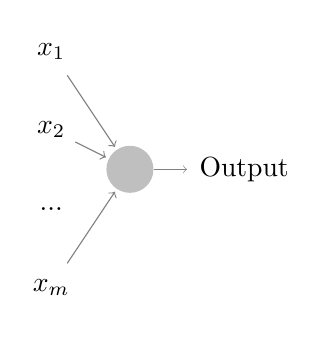
\begin{tikzpicture}[shorten >=1pt,->,draw=black!50, node distance=\layersep]
				\tikzstyle{tata}=[,minimum size=17pt,inner sep=0pt]
			    \tikzstyle{neuron}=[circle,fill=black!25,minimum size=17pt,inner sep=0pt]
			    \tikzstyle{output neuron}=[neuron, fill=red!50];

			    % Input neurons
			    \node[tata] (x1) at (0,-1 cm) {$x_1$};
			    \node[tata] (x2) at (0,-2 cm) {$x_2$};
			    \node[tata] (x3) at (0,-3 cm) {...};
			    \node[tata] (x4) at (0,-4 cm) {$x_m$};
			    
			    % Draw the output layer node
			    \node[neuron,pin={[pin edge={->}]right:Output}] (O) at (\layersep,-2.5) {};

			    % Connect every node in the hidden layer with the output layer
			    \path (x1) edge (O);
			    \path (x2) edge (O);
			    \path (x4) edge (O);

			\end{tikzpicture}
			\caption{Model of an artificial neuron}
			\label{fig:perceptron}
		\end{figure}

		The neurons that appeared later still followed a biologic inspiration as described earlier. Unlike the perceptron, most of these neurons were real-valued and the difference from one to the other resides in its transfer function. We cite here two famous ones :
		\begin{itemize}
			\item The \textbf{sigmoid neuron} which defined by a smooth threshold function:
			$$ \sigma(x) = \frac{1}{1 + e^{-x}} $$
			\item The \textbf{Regression Logistic Unit} (ReLU) which activation function is equal to zero for any negative inputs and equal to its input otherwise. This function got famous with the AlexNet \cite{krizhevsky2012imagenet} where the authors could train a network 4 times quicker than with a usual sigmoid neuron.
			$$ \text{ReLU}(x) = \text{max}(0,x) $$
		\end{itemize}

		Finally, another neuron we'll extensively use in this thesis is the \textbf{Recurrent Neuron}. 


	\section{Neural-network}
		Now that we have neurons, we need a network of them to compose an architecture similar to the brain. The networks we are going to work with are called \textbf{feed-forward} neural-networks. They are the most common ones in the literature. \Fref{fig:feed_forward} is a representation of a two-hidden-layer feed-forward neural-network. As you can see, this model consist of groups of neurons. We denote as layer the group of neurons belonging to the same deepness in the model. Therefore, all the neurons visible on the left in our model, compose the first layer of neurons. It's the input layer. The following layers are called the hidden layers and the last one is the output layer. Some variations exists of this definition, for instance, some outputs of the model might be placed at the same level as some hidden layer.

		Our simple example is also a feed-forward neural-network. It has an input layer fully connected to a hidden layer, which is also fully connected to the output layer. As drawn on the schema with the directions of the arrows, the signal propagates from left to right, from the inputs to the outputs. Because of these two reasons (layers fully connected and single direction signal propagation) our simple example is a feed-forward neural-network.		

		\begin{figure}
			\centering
			\def\layersep{1.5cm}
			\begin{tikzpicture}[shorten >=1pt,->,draw=black!50, node distance=\layersep]
			    \tikzstyle{every pin edge}=[<-,shorten <=1pt]
			    \tikzstyle{neuron}=[circle,fill=black!25,minimum size=17pt,inner sep=0pt]
			    \tikzstyle{annot} = [text width=4em, text centered]


			    %%%%%%%%%%%%%%%%%%%%%%%%%%%%%%%%%%%%%%%%%%%% 
			    %%% DRAW THE NODES
			    %%%%%%%%%%%%%%%%%%%%%%%%%%%%%%%%%%%%%%%%%%%%
			    \foreach \name / \y in {1,...,4}
			        \node[] (I-\name) at (0,-\y) {$x_{i\y}$};

			    \foreach \name / \y in {1,...,5}
			        \path[yshift=0.5cm] node[neuron] (H1-\name) at (\layersep,-\y cm) {};

				\foreach \name / \y in {1,...,7}
			        \path[yshift=1.5cm] node[neuron] (H2-\name) at (\layersep*2,-\y cm) {};   

		       	
			    \node[neuron,pin={[pin edge={->}]right:$p_{i1}$}, right of=H2-3] (O-1) {};
			    \node[neuron,pin={[pin edge={->}]right:$p_{i2}$}, right of=H2-5] (O-2) {};

			    %%%%%%%%%%%%%%%%%%%%%%%%%%%%%%%%%%%%%%%%%%%% 
			    %%% DRAW THE PATHS
			    %%%%%%%%%%%%%%%%%%%%%%%%%%%%%%%%%%%%%%%%%%%%
			    \foreach \source in {1,...,4}
			        \foreach \dest in {1,...,5}
			            \path (I-\source) edge (H1-\dest);

			    \foreach \source in {1,...,5}
			        \foreach \dest in {1,...,7}
			            \path (H1-\source) edge (H2-\dest);

			    \foreach \source in {1,...,7}
			    	\foreach \dest in {1,...,2}
				        \path (H2-\source) edge (O-\dest);

			    % Annotate the layers
			    \node[annot,above of=H2-1, node distance=1cm] (hl) {Hidden layer 2};
			    \node[annot,left of=hl] (hl1) {Hidden layer 1};
			    \node[annot,left of=hl1] {Input layer};
			    \node[annot,right of=hl] {Output layer};
			\end{tikzpicture}
			\caption{Feed-forward neural-network with two hidden layers}
			\label{fig:feed_forward}
		\end{figure}


		It's good to mention that other types of network exits such as the \textbf{recurrent networks}. In these networks, there is directed cycles on the graph which means that a neuron can depends on its own output. This model is considered to be closer to the brain structure but the challenge on training these models isn't state of the art. We won't work on these models.

		\textbf{Symmetrically connected} networks is an other types of network, they are called the "Boltzmann machines". They are symmetrical in the sense that connections between neurons exists in the two directions and the weight on this connections is the same in both directions. Here again, we won't work on these models.


	\section{Forward-propagation}
	\label{sec:forward_propagation}
		The logic route now is to relate our neural-network to the prediction or classification task. Lets consider we have a neural-network. This neural-network has weight vectors and biases initialized for each of its neurons. When we input a vector on the left of this neural-network each neurons on the next layer will be assigned a local output value (given the inputs on the previous layer). Following this same pattern from layer to layer, the input signal (vector $\boldsymbol{x}$) will propagate until the output layer resulting in our prediction.

		\vskip 1cm
		\textit{\textbf{Notation:}}
		To refer to the weights of the $j$th neuron of the $l$th layer we note $\boldsymbol{w}^l_j$. The superscript refer to the layer and the lower-script refer to the neuron number on this layer. Also, we note $b^l_j$ the bias of the $j$th neuron of the $l$th layer. As a sum-up of the inputs, $z^l_j$ is the weighted sum plus bias (${\boldsymbol{w}^l_j}^T x + b^l_j$) of the $j$th neuron of the $l$th layer. Finally, the output of neuron $j$ on layer $l$ is denoted $a^l_j$. \Fref{fig:neuron_notation} sums-up these notations.
		Instead of referring to each and every vectors, we often refer to the matrices composed by the vectors. For instance $W^i$ is the weight matrix composed by each neuron's vectors of the $l$th layer.
		\begin{figure}
			\centering
			\def\layersep{8em}	
			\begin{tikzpicture}[shorten >=1pt,->,draw=black!50, node distance=\layersep]
			    \tikzstyle{every pin edge}=[<-,shorten <=1pt]
			    \tikzstyle{pixel} = []
			    \tikzstyle{neuron}=[circle,fill=black!25,minimum size=17pt,inner sep=0pt]
			    \tikzstyle{annot} = [text width=2em, text centered]
			    \tikzstyle{annot2} = [text width=6em, text centered]
			    
			    %%% DRAW THE NODES
			    \foreach \name / \y in {1,...,3}
			        \node[pixel] (I-\name) at (0,-\y) {};
			    \node (I-4) at (\layersep*.5,-3.5) {$1$};
				\node[neuron] (H-1) at (\layersep*1,-2) {};
				\node[pixel] (O-1) at (\layersep*1.5,-2) {};


			    %%% DRAW THE PATHS
	            \path[every node/.style={sloped}] (I-1) edge node[annot]  {$ w^l_{j;1} $} (H-1);
	            \path[every node/.style={sloped}] (I-2) edge node[annot]  {$ w^l_{j;2} $} (H-1);
	            \path[every node/.style={sloped, anchor=west}] (I-2) edge node[annot2] {$ z^l_j     $} (H-1);
	            \path[every node/.style={sloped}] (I-3) edge node[annot]  {$ w^l_{j;3} $} (H-1);
	            \path[every node/.style={sloped}] (I-4) edge node[annot]  {$ b^l_j   $} (H-1);

	            \path[every node/.style={sloped}] (H-1) edge node[annot]  { $a^l_j$ } (O-1);

			    %%% ANOTATE
			    \node[annot2,above of=H-1, node distance=1cm] () {$j$th neuron on layer $l$};

			\end{tikzpicture}
			\caption{Our notation in a neuron}
			\label{fig:neuron_notation}
		\end{figure}

		\vskip 1cm
		Lets demonstrate this forward-propagation on our simple example. We will propagate $\boldsymbol{x}^1$, the first input sample of the dataset, and get the prediction made by the network. To do so, we need to initialize the weights and biases of the 6 neurons we have. We use weight initialization written on table\ref{tab:NN_weights}.

		\begin{table}[ht]
			\centering
			\begin{tabular}{c|c|c||c|c|c}
				$\boldsymbol{w}^1_1$ & $\boldsymbol{w}^1_2$ & $\boldsymbol{w}^1_3$ & $\boldsymbol{w}^2_1$ & $\boldsymbol{w}^2_2$ & $\boldsymbol{w}^2_3$ \\
				\hline
					$ \left( \begin{matrix} -10  \\ -10  \\  20 \end{matrix}\right) $ &
					$ \left( \begin{matrix} -10  \\  10  \\  10 \end{matrix}\right) $ &
					$ \left( \begin{matrix}  10  \\ -10  \\  10 \end{matrix}\right) $ &
					$ \left( \begin{matrix}  5   \\ -5   \\ -5  \end{matrix}\right) $ &
					$ \left( \begin{matrix} -5   \\  5   \\ -5  \end{matrix}\right) $ &
					$ \left( \begin{matrix} -5   \\ -5   \\  5  \end{matrix}\right) $ \\
				\hline
				\hline
				$b^1_1$ & $b^1_2$ & $b^1_3$ & $b^2_1$ & $b^2_2$ & $b^2_3$ \\
				$-13$   & $-13$   & $-13$   & $0$     & $0$     & $0$     \\
			\end{tabular}
			\caption{ \fref{fig:simple_NN_init} shows the weights on a schema}
			\label{tab:NN_weights}
		\end{table}

		Given these weights, retrieving the prediction of the class of $\boldsymbol{x}^1$ consists on: 
		\begin{itemize}
			\item Propagating $\boldsymbol{x}^1$ through the first neuron layer:
			$$ \sigma(\boldsymbol{z}^1) = \sigma({\boldsymbol{W}^1}^T \boldsymbol{x}^1 + \boldsymbol{b}^1) $$
			$ \sigma \left(
			\left( \begin{matrix} -10 & -10 & 20 \\ -10 & 10 & 10 \\ 10 & -10 & 10 \end{matrix}\right) \cdot
			\left( \begin{matrix} 0  \\ 0  \\ 1  \end{matrix}\right) +
			\left( \begin{matrix} -13 \\ -13 \\ -13 \end{matrix}\right) \right) = 
			\sigma \left( 
			\left( \begin{matrix} 7 \\ -3 \\ -3 \end{matrix}\right) \right) = 
			\left( \begin{matrix} .999 \\ .047 \\ .047 \end{matrix}\right) $
			\item Propagating $\sigma(\boldsymbol{z}^1)$ through the second neuron layer (the prediction layer):
			$$ p(\boldsymbol{z}^1) = \sigma({\boldsymbol{W}^2}^T \sigma(\boldsymbol{z}^1) + \boldsymbol{b}^2) $$
			$ \sigma \left(
			\left( \begin{matrix} 5 & -5 & -5 \\ -5 & 5 & -5 \\ -5 & -5 & 5 \end{matrix}\right) \cdot
			\left( \begin{matrix} .999  \\ .047  \\ .047  \end{matrix}\right) +
			\left( \begin{matrix} 0 \\ 0 \\ 0 \end{matrix}\right) \right) = 
			\sigma \left( 
			\left( \begin{matrix} 9.042 \\ -9.991 \\ -9.991 \end{matrix}\right) \right) = 
			\left( \begin{matrix} .989 \\ .007 \\ .007 \end{matrix}\right) $
		\end{itemize}

		We have here the prediction for $\boldsymbol{x}^1$. To have a percentage out of this prediction we normalize prediction and get that sample $\boldsymbol{x}^1$ could be of class 1 with $98,6\%$ accuracy, could be of class 2 with $.7\%$ or of class 3 with $.7\%$ accuracy. Our simple example, initialized with these weights made an accurate prediction for this sample.
	

	\section{Cost function}
	\label{sec:cost_function}
		Once we have build our model, we consider a cost function, also called "loss function". This cost function define how good is the model doing, considering an evaluation criterion. In the case of classification, we want to evaluate how good the prediction is doing towards the true output.
		The most famous cost functions in neural-network classification are the squared error and the cross entropy (also called the "negative log-likelihood"). For a given sample $i$ with prediction $\boldsymbol{p}^i$ and the true output $\boldsymbol{y}^i$, they are defined as follow:
		\begin{itemize}
			\item Squared error: $$ l(\boldsymbol{p}^i,\boldsymbol{y}^i) = \norm{\boldsymbol{y}^i - \boldsymbol{p}^i}_2^2 $$
			\item Cross entropy: $$ l(\widetilde{\boldsymbol{p}^i},\boldsymbol{y}^i) = -\ln(\widetilde{\boldsymbol{p}^i})^T\cdot{\boldsymbol{y}^i}  $$
		\end{itemize}
		Where $ \tilde{p} $ is the normalized value of the prediction over all the predictions. To evaluate the error of the entire dataset, we use the mean of all the errors. $l(\boldsymbol{P},\boldsymbol{Y}) = \sum_i l(\boldsymbol{p}^i,\boldsymbol{y}^i)$

		\vskip 1cm
		We are going to compute these two errors for the sample one but later on the report, we will only consider the cross entropy.
		\begin{itemize}
			\item Squared error: $$ l(\boldsymbol{p}^1,\boldsymbol{y}^1) =  
									\norm{
									\left( \begin{matrix} .989 \\ .007 \\ .007 \end{matrix}\right) - 
									\left( \begin{matrix} 1    \\ 0    \\ 0    \end{matrix}\right) }_2^2 = 
									.011^2 + .007^2 + .007^2 = .021 $$
			\item Cross entropy: $$ l(\widetilde{\boldsymbol{p}^1},\boldsymbol{y}^1) = 
									- \ln
								 	\widetilde{\left( \begin{matrix} .989 \\ .007 \\ .007 \end{matrix}\right)}^T \cdot 
									\left( \begin{matrix} 1    \\ 0    \\ 0    \end{matrix}\right) = 
									- \ln
								 	\left( \begin{matrix} .986 \\ .007 \\ .007 \end{matrix}\right)^T \cdot 
									\left( \begin{matrix} 1    \\ 0    \\ 0    \end{matrix}\right) = 
									-\ln(.986) = .011
									$$
		\end{itemize}
		
		For the rest of the thesis, we'll be using the cross entropy error function. There is no special motivation under this choice. One mustn't believe that this choice is motivated by $.011$ being lower than $.021$. This result comes from the fact that there are two distinct costs. One compares a distance to the true output (the squared error) whereas cross-entropy gives a negative-log-likelihood.


	\section{Back-propagation}
	\label{sec:back_propagation}
		Until now we've seen how to build a model. We initialized our model with some specific values and propagated an input through this model. The forward-propagation of the signal gave us a prediction that could be compared to the true prediction of the sample thank to a cost function. Given an entire test set, we could use the same cost function to evaluate our model. In this subsection and the following, we investigate on how to modify the model such that it performs better.

		\subsection{Intuition}
			We want the model to perform better. We can't change the input samples nor their true predictions. The only parameters we can change are in the model. We could add neurons and see how new neurons improve the current model but we don't. What we are going to do is to modify the neurons such that they have a positive impact on the error. For each neurons present on the model, we are going to see how a twist on their weights and biases impacts the error made by the model. To find the good twists we use Back-propagation and to take a step in the direction of this twist we use gradient descent (section \ref{sec:gradient_desent}).

			The name of back-propagation comes as the opposite of forward-propagation. We start from the cost ($C=l(\boldsymbol{P},\boldsymbol{Y})$) of the network and see how twisting the weights of the neurons, layer after layers, affects the cost. To be more formal, we search for the direction of the derivative of the cost as a function of the weights and biases of neuron $j$ on layer $i$. To reach this step, we will first consider $\delta^l_i$, the derivative of the cost with respect to the input of neuron $j$ of layer $l$.
			$$ \delta^l_j = \frac{\partial C}{\partial z^l_j } $$
			You might want to watch \fref{fig:neuron_notation} to remind the notation. Also, for notation convenience we'll be using many vector/matrix notations. As a result, we'll use the Hadamard ("$\circ$") and the Kronecker ("$\otimes$") products. The definitions of these two products are reminded in appendix \ref{sec:hadamar_product}.

		\subsection{Step-by-step}
			The \textbf{first} step of back-propagation is to back-propagate the cost $C$ to the last layer $L$.

			\begin{tabular}{c|c}
				\parbox{14em}{
					\begin{equation}
						\begin{split}
							\delta^L_i
							&= \frac{\partial C}{\partial z^L_i } \\
							&= \frac{\partial a^L_i }{\partial z^L_i } \cdot \frac{\partial C}{\partial a^L_i }
						\end{split}
					\end{equation}
				}
				& \parbox{14em}{
					\begin{equation}
						\begin{split}
							\boldsymbol{\delta}^L
							&= \frac{\partial C}{\partial \boldsymbol{z}^L } \\
							&= \frac{\partial \boldsymbol{a}^L }{\partial \boldsymbol{z}^L } \circ \frac{\partial C}{\partial \boldsymbol{a}^L }
						\end{split}
					\end{equation}
				}
			\end{tabular}

			On this last equation, we see that deriving the cost with respect to the neurons' inputs of the last layer $L$ consist on deriving the cost $C$ with respect to the prediction $p$ and on deriving the output of a neuron with respect to it's inputs. 

			The \textbf{second} step is to back-propagate the cost to the other layers $l$. We will here take advantage of the chain rule. 
			\begin{equation}
				\begin{split}
					\boldsymbol{\delta}^l
					&=  \frac{\partial C}{\partial \boldsymbol{z}^l } \\
					&=	\left(\frac{\partial \boldsymbol{a}^l }{\partial \boldsymbol{z}^l }  					\circ\frac{\partial \boldsymbol{z}^{l+1} }{\partial \boldsymbol{a}^l } \right) 	\cdot
					\left(\frac{\partial \boldsymbol{a}^{l+1} }{\partial \boldsymbol{z}^{l+1} }  		\circ\frac{\partial \boldsymbol{z}^{l+2}}{\partial \boldsymbol{a}^{l+1} }\right)  (...)
					\left(\frac{\partial \boldsymbol{a}^L }{\partial \boldsymbol{z}^L } 		 		\circ\frac{\partial C}{\partial \boldsymbol{a}^L }\right) \\
					&=  \left(\frac{\partial \boldsymbol{a}^l }{\partial \boldsymbol{z}^l }  					\circ\frac{\partial \boldsymbol{z}^{l+1} }{\partial \boldsymbol{a}^l }  \right) \cdot
						\left( \frac{\partial \boldsymbol{a}^{l+1} }{\partial \boldsymbol{z}^{l+1} }  	\circ\frac{\partial \boldsymbol{z}^{l+2}}{\partial \boldsymbol{a}^{l+1} }\right) (...)
						\left( \frac{\partial \boldsymbol{a}^L }{\partial \boldsymbol{z}^L }			\circ\frac{\partial C}{\partial \boldsymbol{a}^L }\right) \\
					&= 	\left(\frac{\partial \boldsymbol{a}^l }{\partial \boldsymbol{z}^l }   				\circ\frac{\partial \boldsymbol{z}^{l+1} }{\partial \boldsymbol{a}^l } \right) 		\cdot
						\left( \frac{\partial \boldsymbol{a}^{l+1} }{\partial \boldsymbol{z}^{l+1} }  	\circ\frac{\partial \boldsymbol{z}^{l+2}}{\partial \boldsymbol{a}^{l+1} }\right) (...) 
						\boldsymbol{\delta}^{L}\\
					&= 	\left(\frac{\partial \boldsymbol{a}^l }{\partial \boldsymbol{z}^l }  					\circ\frac{\partial \boldsymbol{z}^{l+1} }{\partial \boldsymbol{a}^l } \right) 	\cdot
						\boldsymbol{\delta}^{l+1}
				\end{split}
			\end{equation}
			At the very end of this equation we see how deriving the cost $C$ with respect to the inputs of layer $l$ depends on the derivative of the next layer, and therefore how back-propagation occurs.

			The \textbf{third} part of the algorithm consist on deriving the cost $C$ with respect to the weights $\boldsymbol{w}^l_j$ and biases $b^l_j$.

			\begin{tabular}{c|c}
				\parbox{14em}{
					\begin{equation}
						\begin{split}
							\frac{\partial C}{\partial \boldsymbol{w}^l_j}
							&= \frac{\partial z^l_j}{\partial \boldsymbol{w}^l_j} \frac{\partial C}{\partial z^l_j} \\
							&= \frac{\partial z^l_j}{\partial \boldsymbol{w}^l_j} \delta^l_j \\
						\end{split}
					\end{equation}
				}
				& \parbox{14em}{
					With $\boldsymbol{z}^l = \boldsymbol{W}^{lT} \boldsymbol{a}^{l-1} + \boldsymbol{b}^l $
					\begin{equation}
						\begin{split}
							\frac{\partial C}{\partial \boldsymbol{W}^l}
							&= \frac{\partial \boldsymbol{z}^l}{\partial \boldsymbol{W}^l} \otimes \frac{\partial C}{\partial \boldsymbol{z}^l} \\
							&= \frac{\partial \boldsymbol{z}^l}{\partial \boldsymbol{W}^l} \otimes {\boldsymbol{\delta}^l} \\
							&= \boldsymbol{a}^{(l-1)T} \otimes \boldsymbol{\delta}^l \\
						\end{split}
					\end{equation}
				}
			\end{tabular}
			\vskip 1em
			\begin{tabular}{c|c}
				\parbox{14em}{
					\begin{equation}
						\begin{split}
							\frac{\partial C}{\partial b^l_j}
							&= \frac{\partial z^l_j}{\partial b^l_j} \frac{\partial C}{\partial z^l_j} \\
							&= \frac{\partial z^l_j}{\partial b^l_j} \delta^l_j \\
						\end{split}
					\end{equation}
				} & \parbox{14em}{
					With $\boldsymbol{z}^l = \boldsymbol{W}^{lT} \boldsymbol{a}^{l-1} + \boldsymbol{b}^l $
					\begin{equation}
						\begin{split}
							\frac{\partial C}{\partial \boldsymbol{b}^l}
							&= \frac{\partial \boldsymbol{z}^l}{\partial \boldsymbol{b}^l} \otimes \frac{\partial C}{\partial \boldsymbol{z}^l} \\
							&= \boldsymbol{\delta}^l \\
						\end{split}
					\end{equation}
				}
			\end{tabular}



		\subsection{Equations applied to our simple example}
			Before applying the back-propagation, we are going to compute some important derivatives. We will differentiate our cross entropy cost $C$ with respect to its inputs and differentiate the sigmoid neurons with respect to their inputs too.
			\begin{itemize}
				\item The \textbf{derivative of the cost} $C$ with respect to the predictions $p_j$:
					\begin{equation}
						\begin{split}
							\frac{\partial C}{\partial a^L_j}
							&= \frac{\partial C}{\partial p_j} \\
							&= \frac{\partial \left( -\ln(\boldsymbol{p})^T \cdot \boldsymbol{y} \right) }{\partial p_j} \\
							&= -\sum_k \left( \frac{y_k \partial \ln(p_k)}{\partial p_k}\frac{\partial p_k}{\partial p_j} \right)\\
							&= -\sum_k \left( \frac{y_k}{p_k}\frac{\partial p_k}{\partial p_j} \right)\\
						\end{split}
					\label{eq:cost_over_pred}
					\end{equation}
				\item The \textbf{derivative of a neuron}'s output $a^l_j$ with respect to its inputs $z^l_j$ (or $\boldsymbol{a}^l$ wrt. $\boldsymbol{z}^l$).
					\vskip 1em
					\begin{tabular}{c|c}
						\parbox{14em}{
							\begin{equation}
								\begin{split}
									\frac{\partial a^l_j}{\partial z^l_j}
									&= \frac{\partial \sigma(z^l_j)}{\partial z^l_j} \\
									&= a^l_j (1-a^l_j)
								\end{split}
							\end{equation}
						}& \parbox{14em}{
							\begin{equation}
								\begin{split}
									\frac{\partial \boldsymbol{a}^l}{\partial \boldsymbol{z}^l}
									&= \frac{\partial \sigma(\boldsymbol{z}^l)}{\partial \boldsymbol{z}^l} \\
									&= \boldsymbol{a}^l \circ (1-\boldsymbol{a}^l)
								\end{split}
							\end{equation}
						}
					\end{tabular}
				\item \textbf{Derivative of the softmax neurons}: In the cost description (section \ref{sec:cost_function}), we mention a normalized input $\widetilde{\boldsymbol{p}}$ but didn't emphasize on it. This normalized input impacts the last layer of the network such that the derivatives of this layer are different than simple sigmoid neurons. That kind of layer is called a softmax layer and is often used when neural-networks when dealing with multi-class tasks. You'll find more information on this function on the "Pattern recognition and machine learning" book \cite{bishop2006pattern} starting on page 113. Right bellow we derive the outputs of these softmax neurons with their aggregated inputs. There is two cases to derive: the first one is when we differentiate the neuron $a^L_j$ with respect to $z^L_j=1$. The second is when we derive the other neurons $a^L_j$ with respect to $z^L_m=0$.
				\begin{itemize}
					\item If $p_j$ is derived from its input $z^L_j$
						\begin{equation}
							\label{eq:softmax_deriv_1}
							\begin{split}
								\frac{\partial a^L_j}{\partial z^L_j}
								&= \frac{\partial p_j}{\partial z^L_j} \\
								&= \frac{\partial (e^{z^L_j}/\sum_k e^{z^L_k})}{ \partial z^L_j} \\
								&= p_j (1-p_j)
							\end{split}
						\end{equation}
					\item IIf $p_j$ is derived from another input $z^L_m$
						\begin{equation}
							\label{eq:softmax_deriv_2}
							\begin{split}
								\frac{\partial a^L_j}{\partial z^L_m}
								&= \frac{\partial p_j}{\partial z^L_m}\\
								&= \frac{\partial (e^{z^L_m}/\sum_k e^{z^L_k})}{ \partial z^L_j} \\
								&= -p_j p_m
							\end{split}
						\end{equation}
				\end{itemize}
			\end{itemize}

			\vskip 1cm
			\textbf{Back-propagate:}\\
			We've seen the result of some derivatives of some functions present in our simple example. These derivatives will help us in applying the back-propagation algorithm. As mentions on the previous section, there is three main steps to take. \textbf{First} differentiate the cost $C$ with respect to the inputs of the last layer. In our case we differentiate the cross entropy function with respect to the inputs of normalized-output-neurons. In other words we derive the cost function with respect to the inputs of the softmax neurons. The \textbf{second} step consist on back-propagating the error layer by layer such that we get the derivative of the cost with respect to the inputs of layer $l$. \textbf{Third}, and last step, is to compute the derivatives at the weights and biases level instead of just the 'input' of the neurons as we've been doing so far.
			\begin{enumerate}
				\item To compute the \textbf{derivative of the cost} with respect to the inputs of the \textbf{softmax layer} we use the results of equations \ref{eq:cost_over_pred}, \ref{eq:softmax_deriv_1} and \ref{eq:softmax_deriv_2}.
					\begin{equation}
						\begin{split}
							\delta^L_j
							&= \frac{\partial C}{\partial z^L_j } \\
							&= \frac{\partial C}{\partial p_j} \frac{\partial p_j}{\partial z^L_j } \\
							&= -\left(\sum_k \frac{y_k}{p_k} \cdot \frac{\partial p_k}{\partial p_j } \frac{\partial p_j}{\partial z^L_j } \right) \\
							&= -\left(\sum_k \frac{y_k}{p_k} \cdot \frac{\partial p_k}{\partial z^L_j } \right) \\
							&= -\left(\sum_{k=j} \frac{y_k}{p_k} \cdot p_k(1 - p_k) \right) - \left(\sum_{k!=j} \frac{y_k}{p_k} \cdot -(p_j p_k) \right) \\
							&= -\left(y_j  (1 - p_j) \right) + \left(\sum_{k!=j} y_k(p_j) \right) \\
							&=  \left(y_j p_j  - y_j\right)  + \left(\sum_{k!=j} y_k p_j  \right) \\
							&=  \left(\sum_{k} y_k p_j  \right) - y_j \\
							&=  p_j - y_j \\
						\end{split}
					\end{equation}
					Which in a vector notation is $\boldsymbol{\delta}^L = \boldsymbol{p} - \boldsymbol{y}$
				\item Then we \textbf{back-propagate} to other layers. We only have two layers, we've just done the last layer $l=2$. We now do layer $l=1$
					\begin{equation}
						\begin{split}
							\boldsymbol{\delta}^{1}
							&= \frac{\partial \boldsymbol{a}^1 }		{\partial \boldsymbol{z}^1 } 		\circ
							\left( \frac{\partial \boldsymbol{z}^2 }	{\partial \boldsymbol{a}^1 } \cdot \boldsymbol{\delta}^2 \right) \\
							&= \frac{\partial \sigma(\boldsymbol{z}^1)}	{\partial \boldsymbol{z}^1}\circ
							\left( \frac{\partial ({\boldsymbol{W}^2}^T \boldsymbol{a}^1 + \boldsymbol{b}^1 )}{\partial \boldsymbol{a}^1} \cdot \boldsymbol{\delta}^2 \right)\\
							&= \sigma(\boldsymbol{z}^1)\circ(1-\sigma(\boldsymbol{z}^1)) \circ ({\boldsymbol{W}^2}^T \cdot \boldsymbol{\delta}^2) \\
							&= \boldsymbol{a}^1 \circ(1-\boldsymbol{a}^1) \circ ({\boldsymbol{W}^2}^T \cdot \boldsymbol{\delta}^2) \\
						\end{split}
					\end{equation}
				\item Finally, we compute the \textbf{derivative of the costs} with respect to the \textbf{weights and biases}.\\
				\begin{tabular}{c|c}
					\parbox{14em}{
						\begin{equation}
							\begin{split}
								\frac{\partial C}{\partial \boldsymbol{W}^2}
								&= \frac{\partial \boldsymbol{z}^2}{\partial \boldsymbol{W}^2} \otimes {\boldsymbol{\delta}^2} \\
								&= {\boldsymbol{a}^1}^T \otimes {(\boldsymbol{p} - \boldsymbol{y})} \\
							\end{split}
							\label{eq:BP_w2}
						\end{equation}
					} & \parbox{14em}{
						\begin{equation}
							\begin{split}
								\frac{\partial C}{\partial \boldsymbol{W}^1}
								&= \frac{\partial \boldsymbol{z}^1}{\partial \boldsymbol{W}^1} \otimes {\boldsymbol{\delta}^1} \\
								&= \boldsymbol{x}^T \otimes {\boldsymbol{\delta}^1} \\
							\end{split}
							\label{eq:BP_w1}
						\end{equation}
					} \\
					\parbox{14em}{
						\begin{equation}
							\begin{split}
								\frac{\partial C}{\partial \boldsymbol{b}^2}
								&= \frac{\partial \boldsymbol{z}^2}{\partial \boldsymbol{b}^2} \otimes {\boldsymbol{\delta}^2} \\
								&= (\boldsymbol{p} - \boldsymbol{y}) \\
							\end{split}
							\label{eq:BP_b2}
						\end{equation}
					} & \parbox{14em}{
						\begin{equation}
							\begin{split}
								\frac{\partial C}{\partial \boldsymbol{b}^1}
								&= \frac{\partial \boldsymbol{z}^1}{\partial \boldsymbol{b}^1} \otimes {\boldsymbol{\delta}^1} \\
								&= \boldsymbol{\delta}^1 \\
							\end{split}
							\label{eq:BP_b1}
						\end{equation}
					}
				\end{tabular}
			\end{enumerate}




	\section{Gradient descent}
	\label{sec:gradient_desent}
		With back-propagation, we've computed the derivatives of the cost with respect to the weights and biases of the model. In other words, we've seen how to twist the neurons' parameters such that, given an input sample, they lower the cost.

		We now want to find the neurons' parameters that will lower the model's cost $C$. We'll search for this value with Gradient Descent. Gradient descent is an iterative algorithm aiming at finding the local minimums of a function. At each steps its improves its chances to be closer to a local minimum.

		\vskip 1em
		Consider a function $f:\mathbb{R}^n\rightarrow\mathbb{R}$ and its gradient $\nabla f$. Gradient descent works by taking advantage of the gradient of the function $f$ at a point $x$ such that, following the negative value of the gradient, the algorithm can find a local minimum for the function. 
		$$ x_{t+1} = x_t - \epsilon \nabla f(x)$$


		On deep learning, we don't use gradient descent but \textbf{Stochastic Gradient Descent (SGD)}. This descent algorithm picks a sample at random on the dataset and evaluate the gradient from it. Still, ”The derivative based on a randomly chosen single example is a random approximation to the true derivative based on all the training data” \cite{elkan2013maximum}.


		\subsection{Example on our simple example}
			We want to perform a step towards a lower cost on our simple example using SGD. We'll pick 'at random' the 1st sample on the training set:
			$$ \boldsymbol{x}^1 = \left( \begin{matrix} 0  \\ 0  \\ 1  \end{matrix}\right) $$
			That is of class $y^1 = 1$. The model we consider is initialized as before. It has the weight and biases of \fref{tab:NN_weights}.

			To perform a step toward a lower cost in the model, we use the prediction made by the current model on this sample $\boldsymbol{x}^1$ (already computed on section \ref{sec:forward_propagation}), and compute the back-propagation equation \ref{eq:BP_w2}, \ref{eq:BP_w1}, \ref{eq:BP_b2}, \ref{eq:BP_b1} with the prediction $\boldsymbol{p}^1$ and output $\boldsymbol{y}^1$.

			Using an epsilon $\epsilon = .5$, we get the following updates : 


			\begin{tabular}{cc}
				$ \boldsymbol{W}^1_{t+1} = \boldsymbol{W}^1_t - \epsilon \frac{\partial C}{\partial \boldsymbol{W}^1} = 
					\left( \begin{matrix}
					-10.0 	& -10.0 	& 10.0 \\
					-10.0 	& 10.0 	& -10.0 \\
					20.0 	& 10.0 	& 10.0 \\
					\end{matrix} \right) - \epsilon 
					\left( \begin{matrix}
					-0.0 	& 0.0 	& 0.0 \\
					-0.0 	& 0.0 	& 0.0 \\
					-0.0 	& 0.003 	& 0.003 \\
					\end{matrix} \right) $ \\
				$ \boldsymbol{W}^1_{t+1} = 
					\left( \begin{matrix}
					-10.0 	& -10.0 	& 10.0 \\
					-10.0 	& 10.0 		& -10.0 \\
					20.0 	& 9.998 	& 9.998 \\
					\end{matrix} \right)$ \\

				\hline
				$ \boldsymbol{W}^2_{t+1} = \boldsymbol{W}^2_t - \epsilon \frac{\partial C}{\partial \boldsymbol{W}^2} = 
					\left( \begin{matrix}
					5.0 	& -5.0 	& -5.0 \\
					-5.0 	& 5.0 	& -5.0 \\
					-5.0 	& -5.0 	& 5.0 \\
					\end{matrix} \right) - \epsilon 
					\left( \begin{matrix}
					-0.013 	& 0.007 	& 0.007 \\
					-0.001 	& 0.0 	& 0.0 \\
					-0.001 	& 0.0 	& 0.0 \\
					\end{matrix} \right) $ \\
				$ \boldsymbol{W}^2_{t+1} = 
					\left( \begin{matrix}
					5.007 	& -5.003 	& -5.003 \\
					-5.0 	& 5.0 	& -5.0 \\
					-5.0 	& -5.0 	& 5.0 \\
					\end{matrix} \right)$ \\


				\hline
				$ \boldsymbol{b}^1_{t+1} = \boldsymbol{b}^1_t - \epsilon \frac{\partial C}{\partial \boldsymbol{b}^1} = 
					\left( \begin{matrix}
					-13.0 \\
					-13.0 \\
					-13.0 \\
					\end{matrix} \right) - \epsilon 
					\left( \begin{matrix}
					-0.0 \\
					0.003 \\
					0.003 \\
					\end{matrix} \right)$ \\
				$ \boldsymbol{b}^1_{t+1} = 
					\left( \begin{matrix}
					-13.0 \\
					-13.002 \\
					-13.002 \\
					\end{matrix} \right)$ \\

				\hline
 				$ \boldsymbol{b}^2_{t+1} = \boldsymbol{b}^2_t - \epsilon \frac{\partial C}{\partial \boldsymbol{b}^2} = 
					\left( \begin{matrix}
					0.0 \\
					0.0 \\
					0.0 \\
					\end{matrix} \right) - \epsilon 
					\left( \begin{matrix}
					-0.013 \\
					0.007 \\
					0.007 \\
					\end{matrix} \right)$ \\
				$ \boldsymbol{b}^2_{t+1} = 
					\left( \begin{matrix}
					0.007 \\
					-0.003 \\
					-0.003 \\
					\end{matrix} \right)$ \\
			\end{tabular}

			As a result, our model moved towards a better one (considering this sample). The loss of this model (toward $x_1$) before the updates was $.0135$ and now is $.0134$. Considering all the samples, the loss was before $.014240$ and decreased to $0.014233$. This gradient descent algorithm helped us lowering the loss made by the model.

	\chapter{Saliency Through Deep Nets} % (fold)
\label{sec:saliency_through_deep_nets}
	
	In this chapter we review the contribution we made on deep learning and contextualize it into our problematic.

	\section{Context of the research}
	\label{sec:context_of_the_research}

		As a reminder, the aim of the thesis is to perform Audio-visual perception for human action recognition and to recognize object affordances from an assistant robot. The research direction we consider to tackle this problem is close-to-real-time semi-supervised learning. To be more specific, we want to teach a classifier to localize human actions, both in time and space, from an incomplete dataset. 	

		\subsection{Video Dataset}
		\label{sub:dataset}
			Going through the existing video datasets, we realized that none of the video datasets had the desired properties of our problematic. The video datasets would be soundless, filmed from high grounds (e.g. video surveillance), filmed with lots of constrains (e.g. same, or very few, people performing actions) and labeled without spatial information. Yet, in September 2016, Youtube released a new database \cite{abu2016youtube} composed by 8 million videos and 4800 classes. All the videos contain a sound band, where filmed from diverse point of views and are very diverse. Regrettably, even for a human (like myself), it's not always obvious to recognize the desired labels of a video, yet, we can expect to find some patterns throughout these classes. One idea could be to shrink this dataset into another one with our desired classes.


		\subsection{Image Dataset}
		\label{sub:image_dataset}
			Before tackling the spatio-temporal analysis of a video stream, we started our researches on spatial analysis of frames (or images). Obviously, these dataset would be composed of images displaying objects frequently used by humans. As we also want to evaluate the localization abilities of our classifier, we also needed our datasets to contain localization labeling. With respect to this constrains, we selected three datasets : Microsoft coco \cite{lin2014microsoft}, ILSVRC2012 \cite{ILSVRC15} and Pascal VOC 2007 \cite{pascalVoc2007}. Each of them includes frequently used objects with both labels and 2D localizations.



		\subsection{Supervised Learning}
		\label{sub:supervised_learning}
			In order to attend the spatial detection of classes, we first have been looking into fully-supervised deep-learning. This method implies that we classify our dataset with a neural network which objective function has as parameters (a) the input image, (b) its class and (c) the localization of this class. Here we found 3 papers :
			\begin{itemize}
				\item \textbf{R-CNN\cite{girshick2014rich} :} In this paper, the authors (a) would perform a selective search on the input image, resulting in 2K images (extracted from the original one). They would then (b) run this images into a convolutional net to obtain a large feature vector and (c) classify these regions with a SVM. Because of the selective search and the propagation of the large amount of images in the network, this implementation wasn't real time, still its mAP reached $66\%$ on VOC2007.
				\item \textbf{Faster R-CNN\cite{ren2015faster} : } In this other paper, Ren et al. would tackle the same problem with a similar approach but they roughly switched the convolution and the selective search. As a result a single image would be (a) processed by a CNN which would produce a feature map. This map would (b) be analyzed by a region proposal network to create region proposals and followed by (c) a classifier to produce the combination of classes and regions. This method was faster (198ms) and its mAP close to $79\%$ on VOC2007.
				\item \textbf{YOLO\cite{redmon2015you} :} Here, Redmon et al. took a different approach on the problem. They would (a) split the original image into 49 equal squares and (b) guess, for each of them, (b.1) a bounding box probability and shape (the bounding box would ofter be larger than the box in which the prediction takes place) and (b.2) the probability of the class included in this box. (c) Given these many values, they would aggregate the results into a prediction. With this simpler architecture, the authors reached $78.6\%$ mAP on VOC2007 and a speed of 25ms.
			\end{itemize}

		\subsection{Semi-Supervised Learning}
		\label{sub:semi_supervised_learning}
			The methodology we prefer to solve our problematic is "deep semi-supervised learning". As we've seen earlier, there is plenty of video datasets that exist (which we could aggregate) but none of them have a spatio-temporal labeling of the classes. What they have instead is a class labeling for the video. What we expect from our work is to localize an unspecified pattern under each and every class which would discriminate a class from another one and which, hopefully, would correspond to a class localization. In their work, Zhou et al. \cite{zhou2015learning} used that kind of technique. Their learning algorithm is a function of two inputs : (a) the image and (b) the class it belongs to. At run time, the classifier is able to predict, close to real-time, a class and its position on the image. Sadly, there wasn't any time or accuracy evaluation on VOC2007 comparison. 
			What we found in the afford mentioned paper, is (a) the model always predict a class. (b) The Tensorflow implementation is sub-optimal and won't work real-time. Still, we believe their technique, based on summed of convolved images (namely : Global Average Polling (GAP)), is very efficient and should be further investigated.


	
	\section{Work on saliency}
	\label{sec:work_on_saliency}

		\subsection{Global Average Pooling}
		\label{sub:global_average_pooling}
			In this section, we want to emphasize the benefits of Global Average Pooling (GAP) as formulated and used in Zhou et al.'s work \cite{zhou2015learning}. GAP is a simple operator performing the mean of a two dimensional tensor into a value. In their paper, the operator was used the following way : consider a stack of 2D convolutions over an image resulting in a 3 dimensional tensor. The GAP operator, applied to this last tensor, would result in a one dimensional tensor which would correspond to the means of each activation unit. Lets $f_k(x,y)$ represent an activation of unit $k$ at spatial location $(x,y)$.
			\begin{equation}
				\text{CAM}_k = \sum_{x,y}f_k(x,y)
			\end{equation}

			Because of its formulation, the values retrieved at the GAP layer are position agnostic. The x's and y's pixels localizations are lost. Thankfully, we can record the 3D tensor preceding the GAP layer and use it to render what Zhou et al. called the Class Activation Mapping, a mapping where we would see the activity of the class.

		\subsection{Class Activation Mapping}
		\label{sub:class_activation_mapping}
			After the GAP, Zhou et al. placed a single neuron for each class $s_c$ which were fed to the softmax function. 
			\begin{equation}
				s_c = \sum_k w_k^c \cdot \text{CAM}_k
			\end{equation}
			The $w_k^c$ weight corresponds to the importance a $f_k$ unit has in recognizing a class. Multiplying one with the other, we can reconstruct a heat-map indicating where was the class active :
			\begin{equation}
				M_c = \sum_k w_k^c \cdot f_k(x,y)
			\end{equation}

		\subsection{Issues}
		\label{sub:issues}
			Much of this work is very satisfying. The classifier is able to detect classes (the learning task) and to provide a saliency map (without location labeling). Yet, we found two issues : 
			\begin{itemize}
				\item the first one is related to the messiness of the prediction when none of the learned classes are present. This may sound silly as the classifier isn't supposed to deal with this type of situation, yet, in our use case, we would like our classifier to be insensible to images with none of the target classes. 
				\item The second issue is more of a conceptual one. By leveraging the $\text{CAM}_x$ values and aggregating them into a single neuron, the classifier looses some spatial dependencies. 
				For the sake of this argument, lets consider the $f_1$ unit was computing the probability of a face being present in an image and $f_3$ was computing the probability of a chest being present. These two probabilities are a function of a given amount of xs and ys pixels, therefore, they are 2D localized. Using weighted neurons after the CAM layer removes the localization relation existing between the chest and the face.
			\end{itemize}
			In the following subsection, we will see how we addressed those two issues.

		\subsection{Second issue}
		\label{sub:second_issue}		
			To address these two issues we run experiments. We first addressed the conceptual one by comparing a regular conv-FC net (a network composed by a stack of convolutional layers followed by fully connected layers and a softmax) to a conv-CAM net (a network composed by a stack of convolutional layers followed by a CAM layer and a softmax). 
			
			The idea was to confirm that the fully connected layer(s) at the end of the Conv-FC were forcing the network to over-fitting the x and y positions of a class while training on a given dataset. Concretely : consider we have to train a classifier to recognize beds and the beds images on the database only shows beds on the lower left corner of these databases. Considering this training setup, we hypothesize that if, at test time, we show to the classifier images with a bed on the top right corner, the classifier won't be able to classify this new sample as a bed.

			We could prove this property (a) mathematically or (b) In practice.

			\textbf{(a) Mathematically}, the intuition would be that the gradient of the target class would never have high values at the "non-active" regions. Considering a Conv-FC net with a single Fully-Connected layer, we would see that the gradients of the detected softmax class would be multiplied to the output values of the last convolutional layer which would be high if their range of attention contains a bed, and low otherwise. With the training algorithm we use (stochastic gradient descent) these low gradients won't allow a class detection where the training set didn't show the desired pattern (a bed elsewhere than the lower left corner to mention our previous example).

			\textbf{(b) In practice}, we've tried to support our argument with an experiment. The first step was trying to determine whether if a Conv-FC net would over-fit to a given position on a constrained dataset. To do this, we simulated a training MNIST dataset \ref{sub:constrained_position_mnist} with images of size $(100*100)$ and the digits at a position $(20*20)$ (right figure of \fref{fig:CP_MNIST_5050_2020_noisy}). At test time, we used a dataset with different digits positions. "Obviously" those images were only correctly classified when the digits were at $(20*20)$. 

			On the following section, we further detail our experiments.

		\subsection{Experiments}
		\label{sub:experiments}
			In this section, we describe the experiments and their results. 

			\textbf{Test-sets :} These results will be composed by two key values which are the Test-Set accuracy "As Trained" (TSAT)(with a digit at the top-left position) and the Test-Set accuracy "With Random Positions" (TSWRP). On the first case TSAT is constructed like the train-set (same image size, same image position, same noise) but the digits are different. On the second case the TSWRP is constructed likewise but the position of the image is selected at random. 
			When nothing is mentioned, we consider the TSAT to be build with the following parameters : $w^{cp}=100,h^{cp}=100, x^{cp}=10,y^{cp}=10$ and a background equals to ten percent of a noise under a uniform law.

			\textbf{Con-nets :}
			Earlier, we mentioned the Conv-FC and the Conv-CAM, most of the times, the convolutional part of these network is as follow :
			\begin{itemize}
				\setlength\itemsep{-0.4em}
				\item conv1\_1 $[3*3*1*16]$ \footnote{[filter height, filter width, input channels, output channels]}
				\item conv1\_2 $[3*3*16*16]$
				\item max-pool
				\item conv2\_1 $[3*3*16*16]$
				\item conv2\_2 $[3*3*16*16]$
				\item max-pool
				\item conv3\_1 $[3*3*16*16]$
			\end{itemize}

			\textbf{Learning parameters :} When not mentioned, we understand that the learning rate of the network is $0.005$, and the optimizer is the default Tensorflow implementation of "RMSprop". Also, we stopped the learning after 10 epochs and report the best of these 10 learning accuracies. This last point could be improve thanks to a learning algorithm that would stop automatically when an over-fitting is detected from the learning and validation accuracies.

			\textbf{visualization :} To visualize our results, we use randomly chose a digit and create 64 images with the digit at 64 different positions (in the 100\*100 image)\footnote{(5,5)(5,10)(5,15)(5,20)...(10,5)(10,10)(10,15)...(40,40)}. We then compute the negative-log-likelihood of each of those images and plot the pre-softmax value of each of them (which lead to values unconstrained between [0,1]). This value is also called the "activation" of the neuron before the softmax. We will refer to this visualization as the multiPos graph. (We acknowledge in this parenthesis the lack of methodology due to the selection of a random digit which should have been fixed for proper comparisons of models...).

			\subsubsection{Conv-FC} 
			\label{ssub:conv_fc}
				The conv-FC network has the convolutional structure aforementioned with a single fully-connected layer on top (fc1 is [252516, 512]\footnote{[input dimension, out dimension]}).
				After 10 epochs, the classifier can recognize the top left digits with $98.88\%$ accuracy on the TSAT but can't recognize digits randomly placed on an image : the TSWRP accuracy is $11.23\%$. On the multiPos graph, we see that the digit "6" is never recognized on the 64 images but when the digit was positioned at (10,10).

				\begin{mdframed}[backgroundcolor = gray!30]
					It's straight forward that this model couldn't generalize the position of a digit.
				\end{mdframed}

			\subsubsection{Conv-CAM}
			\label{ssub:conv_cam}
				The Conv-CAM net has the convolutional structure aforementioned followed by an extra convolutional layer (conv3\_2 is $[3*3*16*10]$) which is followed by a GAP and directly connected the softmax layer.

				After 10 epochs, the accuracy on TSAT is $97.30\%$ and $97.24\%$ on TSWRP. We directly see a gap in between this method and the previous one. On the one hand, the model is now able to recognize a digit randomly positioned on the background, but on the other hand, the model is $1.33$ points less accurate than the previous at recognizing our digits on the TSAT. The following model (section \ref{ssub:conv_cam2}) will be aimed at overcoming this issue.

				\begin{mdframed}[backgroundcolor = gray!30]
					We look at the multiPose graph (\fref{fig:multipose_graph_1}) of this model and notice the randomly generated digit was recognized at every positions. We also notice an activation variation (shaped as a sawtooth) depending on the position of the digit and hypothesize this changes to be caused by the shape reduction operated by the pooling layers. This issue will be further investigated in section \ref{ssub:conv_nopool_l1cam}.
				\end{mdframed}

			\subsubsection{Conv-CAM2}
			\label{ssub:conv_cam2}
				Conv-CAM2 have the same structure as Conv-CAM but the conv3\_2 layer which has twice as much output units as Conv-CAM (conv3\_2 is $[3*3*16*20]$). Before the softmax layer, we mean those 10 pairs of neurons and give them to the softmax layer. The key concept is to double the amount of output units such that each class is supported by 2 neurons. This should increase the amount of representations a digit can have (in other words, to increase its discriminant factor).

				Using such network, the accuracy on TSAT raises to $98.96\%$ and $98.97\%$ on TSWRP. The TSAT and TSWRP accuracies are therefore better with Conv-CAM2 than with the reference model Conv-FC on both datasets. (To be honest, I didn't check if this accuracy increase was "statistically significant").

				\begin{mdframed}[backgroundcolor = gray!30]
					\textbf{(a)} As in the previous model (Conv-CAM), \fref{fig:multipose_graph_1} still show a sawtooth shaped activations from the layer preceding the softmax.

					\textbf{(b)} Another fact one can bring up is the presence of the "relatively high" activations from the non-target classes. what we mean here is that the neurons of non-target classes may fire-up even though the class corresponding to this neuron is not present in the image. we refer to this problem as the "multi-activation issue".

					For example, in \fref{fig:multipose_graph_1} (c) we see that the "red" neuron is firing high values even-though this class is not present in the show image.

					We believe, from the second assumption listed in section \ref{sub:issues}, that it would be nice to lower the activations of the non present classes.

					To address this issue, we test a regularization technique in the following paragraph.
				\end{mdframed}
		

			
			\subsubsection{Conv-L1CAM2}
			\label{ssub:conv_l1cam}
				This model was directly build on top of the preceding one (Conv-CAM2) to address the multi-activation issue aforementioned. The method we propose is a simple L1 regularization placed at the last convolutional layer. 

				If we consider the notation used in section \ref{sub:global_average_pooling} this value would be :
				\begin{equation}
					Conv\_3\_2_{L1} = \sum_{x,y,k}f_k(x,y)
				\end{equation}

				With this regularization term, the accuracy is decreased to $98.48$ on TSAT and $98.42$ on TSWRP. We notice that this regularization term didn't helped us performing better than its non-regularized homologue Conv-CAM2 ($- .48$ percentage points on TSAT and $- .55$ on TSWRP).

				\begin{mdframed}[backgroundcolor = gray!30]
					Even-thought the accuracies are decreased, our expected behavior is reached : \fref{fig:multipose_graph_1} (d) shows the activation for a digit "9". We see that its neuron activation is as least twice higher than the other  activations which are now way closer to 0.

					This example is actually very relevant as digits "9" (red line) and "4" (purple line) are often very competitive.

					To better understand the implications of this method, we should (a) compare the height of the neurons activations with and without this regularization term and (b) see if a threshold can be applied to detect a digit (e.g. a digit is present if its neuron activation is over 8)
				\end{mdframed}
				


			\subsubsection{Conv-NoPool-L1CAM}
			\label{ssub:conv_nopool_l1cam}
				Finally, to have a better understanding of the model we've build so far (Conv-L1CAM2), we try to inhibit the sawtooth shape of the activations occurring when the digits moves around the background. Earlier (in section \ref{ssub:conv_cam}), we've hypothesized this behavior to emerge from the pooling layer. In this model, we remove the last pooling layer to understand analyze if it reduces the neurons activations variations.

				This model is least accurate than any previous ones. After 10 epochs, it has an accuracy of $96.8\%$ on TSAT and $96.91\%$ on TSWRP. The pooling layer is known to regularize the model, and removing it inhibited this property.

				\begin{mdframed}[backgroundcolor = gray!30]
					As expected, removing the pooling layer drastically reduces the activation variation of the neurons' activations. \Fref{fig:multipose_graph_1} (e) shows this sawtooth shape reduction. 

					A new investigation would be to try the method described in \cite{springenberg2014striving}. The authors replaced  pooling layers with convolutions of stride equals to the pooling stride. Their results show equal accuracies with this modification which could also help us.
				\end{mdframed}



			\begin{figure}[h]
				\centering
				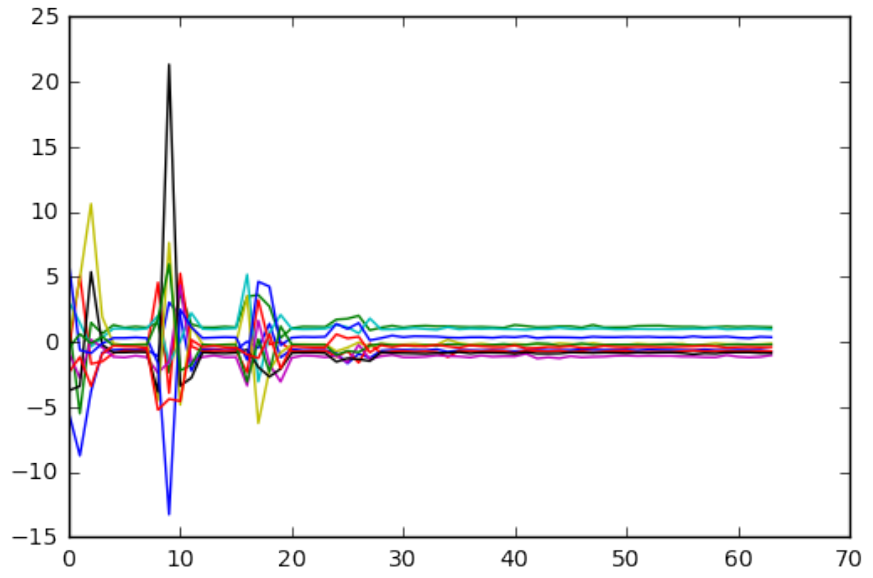
\includegraphics[width=0.45\textwidth]{images/multiPosGraphConvFC}
				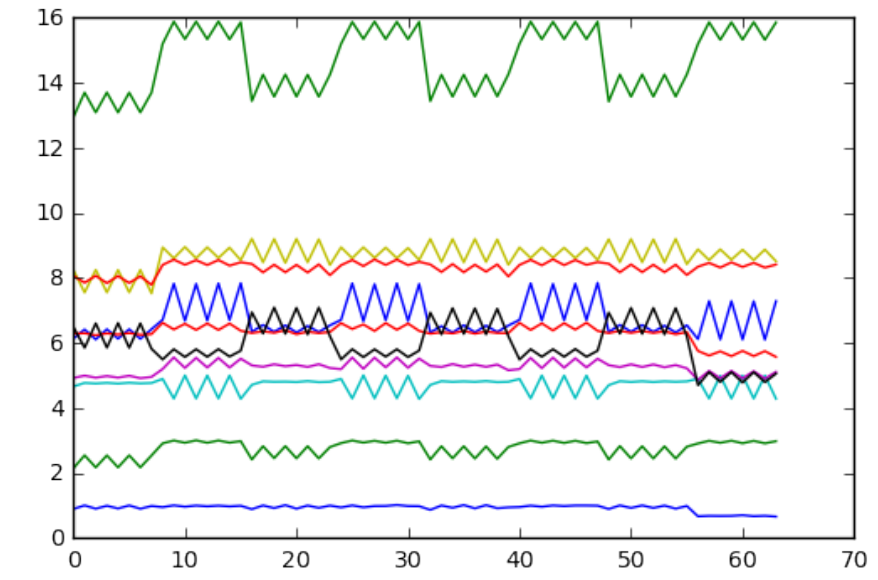
\includegraphics[width=0.45\textwidth]{images/multiPosGraphConvCAM}
				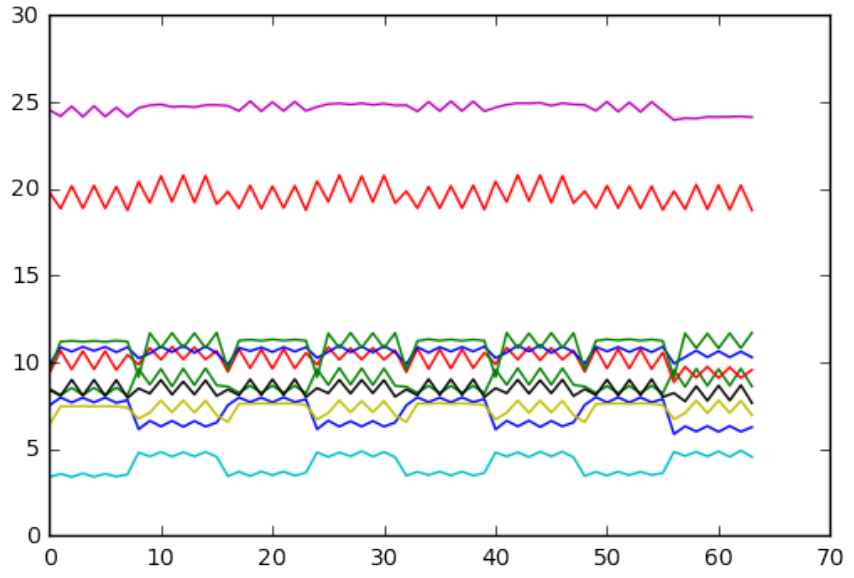
\includegraphics[width=0.45\textwidth]{images/multiPosGraphConvCAM2}
				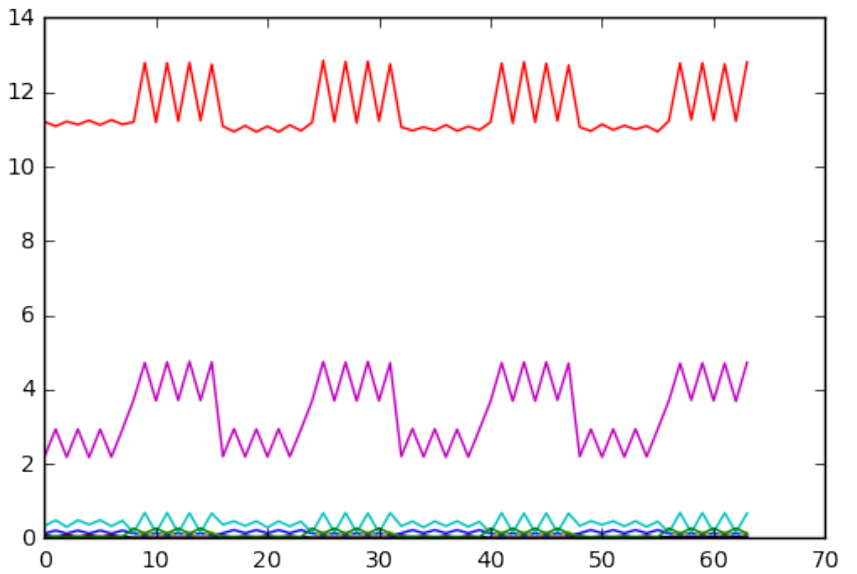
\includegraphics[width=0.45\textwidth]{images/multiPosGraphConvCAM2_L1}
				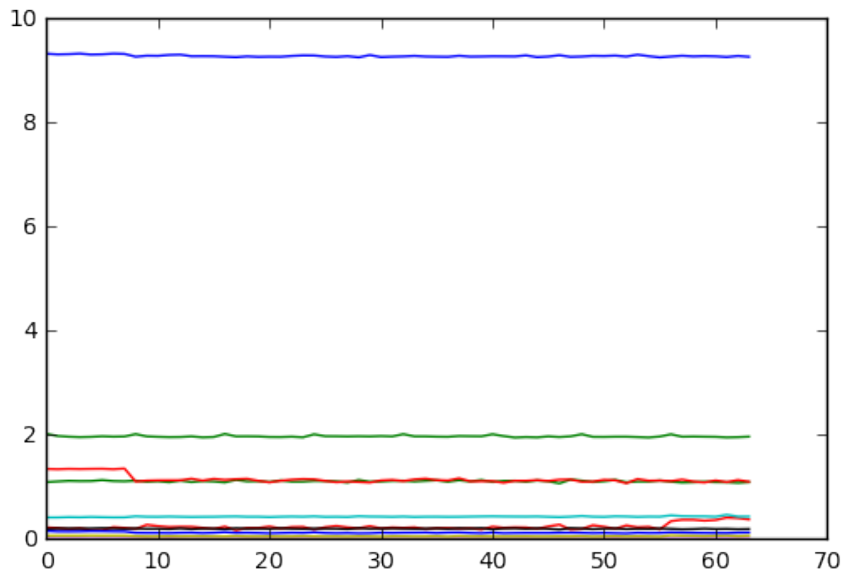
\includegraphics[width=0.45\textwidth]{images/multiPosGraphConvnopool_CAM2_L1}
				\caption{Add an interesting caption...}
				\label{fig:multipose_graph_1}
			\end{figure}

			




			\subsection{Constrained position MNIST}
			\label{sub:constrained_position_mnist}
				We developed a simulated dataset which we refer by Constrained-position MNIST (CP-MNIST). It's simulated in the sense that it's live generated by a piece of code. The main idea is to generate an image that is going to be of a fixed size (224*224 to fit to the literature) and containing an MNIST digit at a position we set $(x^{cp},y^{cp})$. Because we generate this dataset, we have full information on the class label and on the position label. We can further extend this virtual dataset with many informations such as (a) many MNIST sample on one image (e.g. to render numbers) or (b) a video composed by a series of frame (e.g. to render a letter displacement on a 2 or 3 dimensional space). 
				In order to compute this dataset, a few parameters are available :
				\begin{itemize}
					\item The position of the digit : which can be set arbitrarily or randomly with $(x^{cp},y^{cp})$.
					\item The Background size : which is typically set to $(50*50)$ or $(100*100)$ with $(w^{cp},h^{cp})$.
					\item The background type : which can be either zeros (white background) or noisy (random noise from a normal distribution with a parametrized maximum value : $bg$).
				\end{itemize}
				In \fref{fig:CP_MNIST_5050_2020_noisy}, you can see extracts of this virtual dataset.
				\begin{figure}[h]
					\centering
					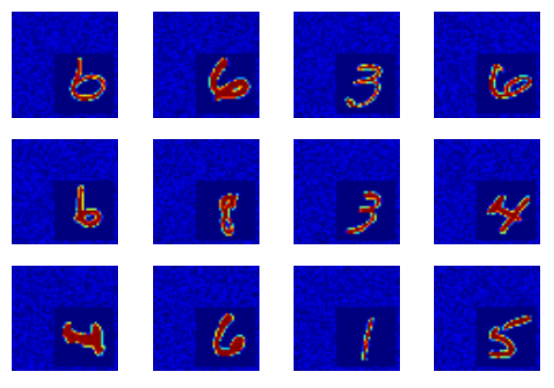
\includegraphics[width=0.45\textwidth]{images/CP_MNIST_5050_2020_noisy} 
					.
					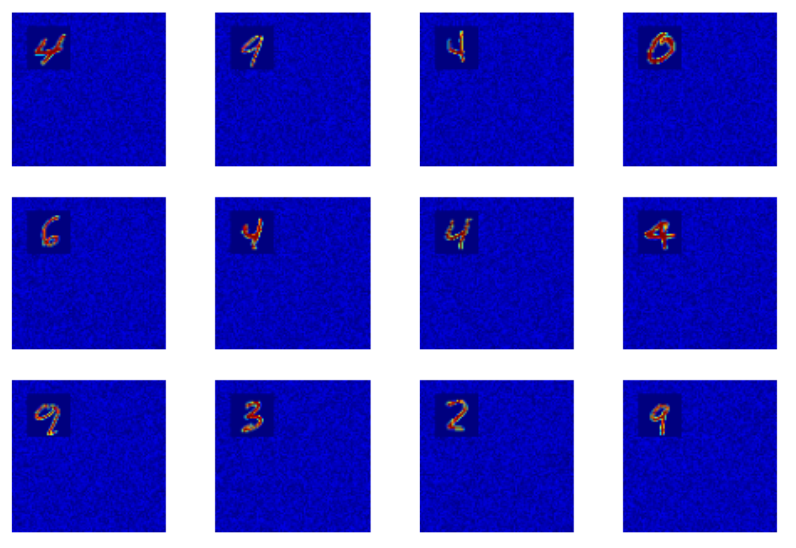
\includegraphics[width=0.45\textwidth]{images/CP_MNIST_100100_2020_noisy}
					\caption{on the left : CP-MNIST generated with : $w^{cp}=50,h^{cp}=50, x^{cp}=20,y^{cp}=20$ and $bg=.1$. and on the right : CP-MNIST generated with : $w^{cp}=100,h^{cp}=100, x^{cp}=20,y^{cp}=20$ and $bg=.1$}
					\label{fig:CP_MNIST_5050_2020_noisy}
				\end{figure}

			
			
			\subsubsection{Regularization term}
			\label{ssub:regularization_term}


			\subsubsection{All Convolutional Net}
			\label{ssub:all_convolutional_net}

			
			


	In this paper, we want to emphasize the use CAM layers for their saliency and localization properties.
	The network we use is therefore a variant to the original network zhou2015learning. In the original paper, the authors introduce a combination of Global Average Pooling, followed by a weighted average and a softmax to classify their images. Here, we investigate the use of Global Average Pooling directly followed by a softmax function to classify our data. With this structure, this new network should capture further informations on spatial relations that the original could not grasp.

	\subsection{Methodology} % (fold)
	\label{sub:methodology}

		Deploy a VGG16 with CAM 
		Deploy a VGG16 with CCN + regularizer + multiple CCN sizes
		Compare each of them on pascal VOC

	\subsection{Results:} % (fold)
	\label{sub:results_}
		
		\begin{itemize}
			\item The detector is position agnostic (Vs FCNN) from training to testing.
			\item Can be use with variable image shapes.
			\item May be use for "one shot" learning of given classes.
		\end{itemize}

	A general comment we can make on both the original model and ours, is that both of the models are training-position-agnostic. What we mean here is that both networks can generalize the concept of an object independently of their position in the training set. If we consider a classification task where the network has to classify shoes against many other other classes, and a set of images randomly chosen from the web, it's very likely that all the images display these shoes at the bottom of the image.\\
	The learned distribution (by the network), and a-priori would be fine, if we were to test our networks on the same type of dataset (randomly chosen from the web) but could present weaknesses if we were to test this network on a dataset without this probability distribution (eg: pictures grabed from a mobile platform, like a humanoid robot, or a fying drone).

	% \chapter{Deep Learning Techniques} % (fold)
\label{sec:deep_learning_techniques}

% section deep_learning_techniques (end)


In the deep learning field, there is a large amount of techniques available to train our networks. These techniques often come with parameters to set. In the following section we are going to see different techniques used to train the networks and the impact of their parameters.

\section{Batch Normalization} % (fold)
\label{sec:batch_normalization}
	
	Batch normalization \cite{ioffe2015batch} was introduced in 2015. 
	The intended outcome of this technique is to favor the back propagation of the gradients. 
	The intuition behind this technique is to avoid plateauing regions of non-linear activation functions by re-centering the inputs to these functions. 
	In order to get the best out of this technique, one should set two parameters. The first one is the size of the batch and the second one is the learning rate. In their paper, Ioffe et al. demonstrate how the learning rate could be increased to speed-up the convergence of their training example, without diverging.
	% \chapter{Saliency Through Deep Nets} % (fold)
\label{sec:saliency_through_deep_nets}
	
	In this paper, we want to emphasize the use CAM layers for their saliency and localisation properties.
	The network we use is therefore a variant to the original network zhou2015learning. In the original paper, the authors introduce a combination of Global Average Pooling, followed by a weighted average and a sotfmax to classify their images. Here, we investigate the use of Global Average Pooling directly followed by a softmax function to classify our data. With this structure, this new network should capure further informations on spatial relations that the original could not grasp.

	\subsection{Methodology} % (fold)
	\label{sub:methodology}

		Deploy a VGG16 with CAM 
		Deploy a VGG16 with CCN + regularizer + multiple CCN sizes
		Compare each of them on pascal VOC

	\subsection{Results:} % (fold)
	\label{sub:results_}
		
		\begin{itemize}
			\item The detector is position agnostic (Vs FCNN) from training to testing.
			\item Can be use with variable image shapes.
			\item May be use for "one shot" learning of given classes.
		\end{itemize}

	A general comment we can make on both the original model and ours, is that both of the models are training-position-agnostic. What we mean here is that both networks can generalize the concept of an object independently of their position in the training set. If we consider a classification task where the network has to classify shoes against many other other classes, and a set of images randomly chosen from the web, it's very likely that all the images display these shoes at the bottom of the image.\\
	The learned distribution (by the network), and a-priori would be fine, if we were to test our networks on the same type of dataset (randomly chosen from the web) but could present weaknesses if we were to test this network on a dataset without this probability distribution (eg: pictures grabed from a mobile platform, like a humanoid robot, or a fying drone).
	


	

	\bibliographystyle{plain}
	\bibliography{papers}


\end{document}



